% ****** Start of file apssamp.tex ******
%
%   This file is part of the APS files in the REVTeX 4 distribution.
%   Version 4.0 of REVTeX, August 2001
%
%   Copyright (c) 2001 The American Physical Society.
%
%   See the REVTeX 4 README file for restrictions and more information.
%
% TeX'ing this file requires that you have AMS-LaTeX 2.0 installed
% as well as the rest of the prerequisites for REVTeX 4.0
%
% See the REVTeX 4 README file
% It also requires running BibTeX. The commands are as follows:
%
%  1)  latex apssamp.tex
%  2)  bibtex apssamp
%  3)  latex apssamp.tex
%  4)  latex apssamp.tex
%
\documentclass[prb,aps,twocolumn,preprintnumbers,amsmath,amssymb]{revtex4}
%\documentclass[preprint,showpacs,preprintnumbers,amsmath,amssymb]{revtex4}

% Some other (several out of many) possibilities
%\documentclass[preprint,aps]{revtex4}
%\documentclass[preprint,aps,draft]{revtex4}
%\documentclass[prb,twocolumn,showpacs,preprintnumbers,amsmath,amssymb]{revtex4}% Physical Review B

\usepackage{graphicx}% Include figure files
\usepackage{dcolumn}% Align table columns on decimal point
\usepackage{bm}% bold math
\usepackage[utf8]{inputenc}
\usepackage[spanish,es-tabla]{babel}
\usepackage{url}
\newcolumntype{P}[1]{>{\centering\arraybackslash}p{#1}}
\newcolumntype{M}[1]{>{\centering\arraybackslash}m{#1}}


\begin{document}

\title{Microondas}% Force line breaks with \\

\author{Alejandro Hernández A.}%
 \email{a.hernandez105@uniandes.edu.co}
\author{Daniel Sánchez M.}%
 \email{d.sanchez462@uniandes.edu.co}
\affiliation{%
Departamento de Física\\ Universidad de los Andes, Bogotá, Colombia.\\
}%

\date{15 de octubre de 2015}% It is always \today, today,
             %  but any date may be explicitly specified

\begin{abstract}
Este informe presenta los datos obtenidos al medir la intensidad de las micoondas recibidas en distintas configuraciones de una fuente emisora y un receptor. Básicamente, se trataron de verficar diversos conceptos vistos en el curso de \textbf{ONDAS Y FLUIDOS} tales como la ley de reflexión, la ley de Snell, ondas estacionarias y patrones de interferencia. Entre los resultados notables cabe mencionar OJO y OJO. Los demás resultados y todos los comentarios de los mismos se muestran en la sección de \textbf{RESULTADOS Y ANÁLISIS}.\\

\noindent \textbf{Conceptos clave:} Microondas, reflexión, refracción, leyes de Snell, ondas estacionarias, patrón de interferencia.
\end{abstract}
                             
\maketitle

\section{INTRODUCCIÓN}
Las leyes de Maxwell, junto con la ley de Lorentz describen completamente la teoría electromagnética clásica. Precisamente, la existencia de las ondas electromagnéticas, de las cuales las microondas forman parte del espectro de alta frecuencia, fueron predichas por Maxwell en el año de 1864 a partir de las susodichas 4 ecuaciones de Maxwell. Por su parte, la verificación experimental de las mismas se dio en el año de 1888 cuando Heinrich Rudolf Hertz demosstró la existencia de las ondas electromagnéticas mediante la contrucción de un aparato para generar y detectar ondas de radiofrecuencia, que consistía básicemtne de un oscilador (generador de ondas) y de un resonador (receptor).\\

Allende de lo mencionado anteriormente, a partir de las leyes de Maxwell se pueden deducir dos de las leyes más famosas de la óptica, a saber, la ley de reflexión \cite{Griffiths}:

\begin{equation}
\label{eq:reflexion}
\theta_I = \theta_R
\end{equation}

y la ley de refracción, usualmente aludida como ley de Snell en honor a su descubridor, el matemático holandés Willebrord Snel van Royen \cite{Griffiths}: 

\begin{equation}
n_1\sin{\theta_I} = n_2sin{\theta_T}
\label{eq:snell}
\end{equation}

Donde $\theta_R, \theta_T$ hacen referencia a los ángulos de reflexión y refracción respectivamente, los cuales, al igual que el ángulo de incidencia, están definidos con respecto a la normal de la superficie de incidencia, por lo que solo pueden tomar valores en $[0,\frac{\pi}{2})$. Por otra parte, el índice de refracción $n$ se define como la razón entre la velocidad de la luz y la velocidad en el medio actual, y está relacionado con la densidad óptica del medio:

\begin{equation}
n = \frac{c}{v} = \sqrt{\frac{\epsilon\mu}{\epsilon_0\mu_0}}
\label{eq:indice}
\end{equation}

Donde $\epsilon$, $\mu$ representan,  respectivamente, la permitividad eléctrica y le permeabilidad magnética del medio, mientras que $\epsilon_0$, $\mu_0$ respresentan las mismas cantidades pero para el vacío. Cabe resaltar que la ley del plano de incidencia, la cual establece que el rayo incidente, el reflejado y el transmitido se encuentran en un mismo plano que es perpendicular a la interfaz, es la que permite caracterizar completamente las direcciones del fenómeno de refracción y reflexión solo con los tres ángulos mencionados previamente.\\

De la ley de refracción cabe resaltar que si el medio de incidencia es más denso ópticamente que el medio de transmisión, existirá un ángulo de incidencia en el intervalo $[0,\frac{\pi}{2})$, tal que el ángulo de refracción tenga que ser exactamente $\frac{\pi}{2}$ para poder satisfacer la ley de Snell. Esta relación se expone en la ecuación \eqref{eq:crit}. Con un posterior análisis sobre los coeficientes de transmisión y reflexión, que indican qué tanta luz se refleja y qué tanta luz se transmite, se puede concluir que para ángulos menores a este ángulo crítico, toda la luz es reflejada, y nada se transmite al otro medio. En estos casos, el ángulo de transmisión tendría que ser mayor a $\frac{\pi}{2}$ o menor a $0$, lo cual no cumple lo asumido por la ley del plano de incidencia. Este es el principio sobre el cual se basa el funcionamiento de la fibra óptica. Aquí, la fibra es tan delgada que el ángulo de incidencia siempre es menor que el ángulo crítico, por lo que siempre se da la reflexión interna total y no se pierde luz por transmisión.

\begin{equation}
\sin{{\theta_I}_{crit}} = \frac{n2}{n1}\sin{\frac{\pi}{2}} < 1
\label{eq:crit}
\end{equation}

Ahora bien, para un conductor perfecto el campo en su interior es nulo \cite{Griffiths}, dado que cualquier campo que se intente aplicar, moverá las cargas en la superficie del conductor de tal manera que lo anule. En este sentido, si se tiene una rejilla de un material conductor, se puede puede dejar pasar campo eléctrico solo en la dirección de la rejilla, dado que la componente del campo que no sea paralela, encontrará el conductor y se anulará. En este sentido, con una rejilla metálica se puede polarizar una onda electromagnética.\\

Si se se tiene luz polarizada incidente a un polarizador con un desfase en la dirección de polarización dado por $\theta_1$ respecto a la luz incidente, teniendo en cuenta que solo puede pasar la componente de campo eléctrico paralela al polarizador, la intensidad de la luz recibida estará dada por:

\begin{equation}
I = \frac{1}{2}\epsilon_0{E^{\parallel}}^2 = \frac{1}{2}\epsilon_0{E_0}^2{\cos^2{\theta_1}} \propto \cos^2{\theta_1}
\label{eq:polarizador}
\end{equation}

Si se pone otro polarizador en medio de estos dos, con desfase $\theta_2$ con respecto a la luz incidente, la intensidad estará dada al aplicar \ref{eq:polarizador} dos veces, teniendo en cuenta que el desfase entre los dos polarizadores es $\theta_1-\theta_2$:

\begin{equation}
\small
I = \frac{1}{2}\epsilon_0{E_0}^2{\cos^2{\theta_2}}\cos^2{ \left( \theta_1-\theta_2 \right) } \propto \cos^2{ \theta_1}\cos^2{ \left( \theta_1-\theta_2 \right) }
\label{eq:polarizador2}
\end{equation}

Nótese que si la luz incidente es perpendicular al polarizador, si solo tenemos en cuenta un polarizador, $\theta_1 = \frac{\pi}{2}$ entonces la onda transmitida tendrá intensidad nula. sin embargo, si ponemos otro polarizador en medio, tendremos de forma general $\theta_1 - \theta_2 \neq \frac{\pi}{2}$ por lo que la onda transmitida no necesariamente tendrá intensidad nula.\\

Aparte de lo mencionado anteriormente, otro experimento que se realizó durante la práctica fue el de 	doble rendija. Si se hace incidir luz monocromática coherente sobre una placa conductora (no deja pasar luz) con una rendija doble con una separación $d$, se observará un patrón de difracción. Este patrón ondulatorio se debe al principio de superposición del campo electromagnético, el cual dice que el campo electromagnético en un punto debido a dos fuentes es la suma de los campos producidos por cada fuente por separado en dicho punto \cite{Griffiths}. Debido a esto, si consideramos ondas, la suma de ambos campos es dependiente de la fase. Si se hace un análisis de los caminos que toman las ondas que pasan por cada una de las rendijas se llegará a la conclusión de que la interferencia destructiva se da cuando:

\begin{equation}
d\sin{\theta} = n\lambda
\label{eq:interferencia}
\end{equation}

Donde $\theta$ se refiere al ángulo respecto al centro de la rejilla de difracción donde se toma la medida de intensidad de la luz.\\

Con el experimento de la doble rendija se puede introducir al campo de la interferometría, donde se busca medir distancias del orden de la longitud de onda con la que se trabaja, al mirar la patrones de interferencia o simplemente la distancia entre los máximos o mínimos que ocasiona la superposición de dos haces de luz que han tomado caminos diferentes. El principio de interferencia por diferencia de fases de haces de luz es el principio detrás de experimentos importantes actuales como los detectores de ondas gravitacionales, y de experimentos que hicieron historia como el de Michelson-Morley.\\

Una de las formas de hacer interferometría con ondas esféricas es el espejo de Lloyd. En dicho experimento se tiene un material conductor paralelo a la dirección emisor-receptor, situado a mitad de camino entre estos dos instrumentos, cuya distancia perpendicular se puede variar para provocar interferencia entre la onda que se refleja en el conductor y la onda que toma el camino emisor-receptor. Un análisis sencillo de la diferencia de caminos, asumiendo que la onda se propaga esféricamente, nos dice que hay interferencia constructiva cuando se tiene:

\begin{equation}
D-2{\left(d^2 + {\left(\frac{D}{2}\right)}^2\right)}^\frac{1}{2} = n\lambda
\label{eq:Lloyd}
\end{equation}

Donde $D$ es la distancia del receptor al emisor, $d$ es la distancia del espejo al centro de la trayectoria, $\lambda$ es la longitud de onda de la luz incidente, y $n$ es un entero.\\

De este experimento de interferometría se puede notar claramente que la condición de interferencia no es lineal, y que además, al alejar el espejo, se disminuye la intensidad de la onda que se refleja (asumiendo que se propaga esféricamente), lo cual altera un poco la condición de interferencia.\\

Un experimento de interferometría que no es afectado por estos factores de no linealidad y de variación de la intensidad, es el interferómetro de Michelson y el de Fabry-Perot. Estos interferómetros trabajan bajo el mismo principio y lo único que los diferencia es el ordenamiento espacial de los elementos. El experimento de Michelson es mostrado en la figura \ref{fig:intmichelson} y consiste en superponer dos haces de luz que han tomado distintos caminos con la ayuda de un material semi-transparente. El de Fabry-Perot es análogo (figura \ref{fig:fabryperot}, sin embargo, los materiales semi-transparentes no están dispuestos a $45^o$ sino en medio del receptor y el transmisor.  En este caso, la relación de interferencia para máximos es simple de deducir y simple en general:\\

\begin{equation}
d = n\frac{\lambda}{2}
\label{eq:Michelson}
\end{equation}

Donde $d$ es la distancia a la que se corre el receptor o el emisor , entre dos máximos o mínimos. \\

De esta manera, muchos otros fenómenos ópticos pueden ser caracterizados con la teoría electromagnética clásica, sin embargo, no es objetivo de este informe describirlos todos .\\ 

\section{Montaje Experimental}

En general el montaje consistía de un emisor, un receptor y un goniómetro que se ubicaron en distintas configuraciones para realizar los diversos experimentos sugeridos en la guía proporcionada para la práctica. Los elementos más importantes del mismo semuestran en la figura \ref{fig: montaje} Es preciso aclarar que no se realizaron todos los experimentos puesto que no se disponía de toda la indumentaria necesaria para la realización de los mismos. Los experimentos que no se realizaron se mencionan a continuación:

\begin{itemize}
	\item \textbf{Experimento 9: Fiber Optics} \\No se disponía de las "tubular plastic bags".
	
	\item \textbf{Experimento 12: Bragg Difraction} \\ No se disponía del cubo que generaba la difracción de las ondas.
\end{itemize}

\begin{figure}[h!]
	\centering
	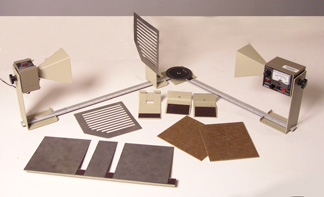
\includegraphics[width=0.5\textwidth]{montaje}
	\caption{ Montaje experimental usado en la práctica. }
	\label{fig: montaje}
\end{figure}

El montaje específico para cada uno de los experimentos se describe a continuación.

\subsection{Reflexión de Microondas}
Para esta manipulación, se configuró el montaje que se muestra en la figura \ref{fig:reflexion} .\\

\begin{figure}[h!]
\centering
\includegraphics[width=0.5\textwidth]{}
\caption{Montaje experimental para la refelxión de Microondas}
\label{fig:reflexion}
\end{figure}

A continuación, dejando el emisor de ondas fijo, a un ángulo de $45^o$ con respecto a la normal del reflector, se procedió a mirar para qué ángulo el receptor mostraba una señal máxima. Se encontró que $45^o$ era el máxmimo de la señal. Esto se hizo para verificar el montaje. \\

Acto seguido, la intensidad del receptor se ajustó en 30X para asegurarse de detectar las más pequeñas variaciones, y se procedió a mover el ángulo incidente desde $20^o$ a $90^o$. El receptor se movió angularmente hasta detectar un máximo. De allí se pudo inferir la relación entre el ángulo incidente y el ángulo reflejado.  \\

Debe anotarse que dado que las ondas son esféricas, hay una medición extra dado que la onda recibida por detector no es sólamente la reflejada sino también se suma una porción directamente proveniente del emisor.\\

\subsection{\label{sec:level2}Refracción a través de un prisma}

Para esta manipulación se configuró el montaje mostrado en la figura \ref{fig:refraccion}. El compartimiento triangular del centro actuaba como prisma. \\

\begin{figure}[h!]
\centering
\includegraphics[width=0.7\linewidth]{Pictures/refraccion}
\caption{Montaje Experimental - Refracción por prisma}
\label{fig:refraccion}
\end{figure}
 
En primer lugar, se procedió a determinar la influencia de este material en la señal del receptor y una vez demostrado que la diferencia era prácticamente nula, se rellenó el interior del prisma con partículas de estireno.\\ 

Con el emisor de ondas fijo, se procedió a mover el detector hasta detectar un máximo en la señal.  Se denota, $ \theta $ el ángulo que marca directamente el detector con el goniómetro. \\

Una vez hallado este ángulo, con el diagrama de la figura \ref{fig:refraccion} se pueden determinar los ángulos incidente y refractado y así hallar el coeficiente de refracción del estireno por medio de la Ley de Snell. \\

En este caso, el medio incidente es el estireno.\\
 
\subsection{\label{sec:level2}Polarización}

Este experimento tuvo dos partes. En primer lugar, el montaje consistía en el que se muestra en la figura \ref{fig:polarizador1} con la excepción de que no había una rejilla de polarización en el medio. Con esto, receptor y emisor frente a frente se procedió a mover el cuerno del detector de ondas dejando el receptor fijo. De esta manera, las ondas producidas impactarían el detector con diferentes ángulos de polarización. \\ 

\begin{figure}[h!]
\centering
\includegraphics[width=0.7\linewidth]{Pictures/polarizador1}
\caption{Montaje Experimental - Polarización}
\label{fig:polarizador1}
\end{figure}

Se midieron así, en aumentos de $5^o$ las señales recibidas para un rango de ángulos de polarización entre $0^o$ y $90^o$. \\

En la segunda parte se prepararon el emisor y el receptor con direcciones paralelas de polarización, se incluyó la rejilla de polarización imitando el montaje en la figura \ref{fig:polarizacion}, y ésta se ubicó en ángulo de $0^o$,$22.5^o$,$45^o$, $67.5^o$ y $90^o$ con respecto al ángulo del emisor. Luego se  se repitieron las medidas para $0^o$, $45^o$ y $90^o$, esta vez configurando el emisor y el receptor en direcciones perpendiculares de polarización.\\ 

\begin{figure}[h!]
\centering
\includegraphics[width=0.7\linewidth]{Pictures/polarizacion}
\caption{Montaje Experimental - Polarización 2}
\label{fig:polarizacion}
\end{figure}

\subsection{\label{sec:level2}Determinación de $ \lambda $}
\textit{Interferencia de doble rendija} \\

\begin{figure}[h!]
\centering
\includegraphics[width=0.7\linewidth]{Pictures/Interferencia}
\caption{Montaje Experimental - Interferencia a Doble Rendija}
\label{fig:Interferencia}
\end{figure}

En este experimento se armó el montaje mostrado en la figura \ref{fig:Interferencia}. Dejando el emisor de ondas fijo, se movió el detector a través del ángulo $ \theta $ mostrado en la figura. Para un barrido de este ángulo entre $0^o$ y $85^o$ en aumentos de $5^o$, se anotó el valor de la intensidad detectada por el receptor. \\

Se repitieron las medidas cambiando la distancia de separación entre rendijas.\\ 

\textit{Ondas estacionarias} \\

Para medir ondas estacionarias se utilizó como reflector el detector mismo. Se ubicaron frente a frente ambos equipos como se muestra en la figura \ref{fig:estacionarias}. \\

\begin{figure}[h!]
\centering
\includegraphics[width=0.7\linewidth]{Pictures/estacionarias}
\caption{Montaje Experimental - Ondas estacionarias}
\label{fig:estacionarias}
\end{figure}

A continuación, se ubicó el detector en donde éste mostrara la lectura de un máximo, y acto seguido se procedió a deslizar el detector hacia atrás. En dos manipulaciones diferentes, se contaron 20 y 30 máximos respectivamente y se procedió a determinar $ \lambda $ con la fórmula para los máximos de una onda estacionaria, la cual es la misma condición presentada en la ecuación \ref{eq:Michelson}. \\ 

\textit{Espejo de Lloyd} \\

Para determinar $ \lambda $ se utilizó también el montaje del espejo de Lloyd mostrado en la figura \ref{fig:espejo}. En este caso el receptor mostrará una señal máxima cuando ambos caminos recorridos por la onda emitida estén en fase. \\

\begin{figure}[h!]
\centering
\includegraphics[width=0.7\linewidth]{Pictures/espejo}
\caption{Montaje Experimental - Espejo de Lloyd}
\label{fig:espejo}
\end{figure}

Para medir este fenómeno se dejan reflector y emisor fijos, separados a una distancia idéntica desde el centro del sistema y se desplaza el reflector hacia atrás. \\

En primer lugar, debe ubicarse el reflector en el primer mínimo que sea posible detectar y acto seguido desplazarlo hacia atrás hasta encontrar cuando menos 10 mínimos de intensidad. De esta forma, la diferencia de caminos debe cumplir la ecuación \ref{eq:Lloyd} para producir interferencia constructiva\\

La medición se realizó dos veces para diferentes separaciones entre emisor y receptor.\\


\textit{Interferómetro de Fabry-Perot} \\

En este caso se recreó el interferómetro de Fabry-Perot, haciendo uso del montaje mostrado en la figura \ref{fig:fabryperot}. Durante esta manipulación se pretendía encontrar la longitud de onda así que se procedió de manera similar al experimento de ondas estacionarias y al espejo de Lloyd.\\


\begin{figure}[h!]
\centering
\includegraphics[width=0.7\linewidth]{Pictures/fabryperot}
\caption{Montaje Experimental - Interferómetro de Fabry-Perot}
\label{fig:fabryperot}
\end{figure}

Dejando el emisor fijo se ubicó el receptor en un mínimo. Acto seguido, se procedió a mover el mismo hacia atrás hasta haber pasado por n mínimos de intensidad. Así pues, con la fórmula \ref{eq:Michelson}, se determinó la longitud de onda. \\ 

\textit{Interferómetro de Michelson} \\

En este experimento se trató de recrear el experimento de Michelson-Morley con microondas, haciendo uso del montaje mostrado en la figura \ref{fig:intmichelson}. \\

\begin{figure}[h!]
\centering
\includegraphics[width=0.7\linewidth]{Pictures/intmichelson}
\caption{Montaje Experimental - Interferómetro de Michelson}
\label{fig:intmichelson}
\end{figure}

Se ubicó el detector en el mínimo más cercano encontrado con respecto al centro del sistema y se procedió a deslizar el equipo hacia atrás contando mínimo diez mínimos de intensidad. Con una fórmula similar a las utilizadas anteriormente, se determinó $ \lambda $. \\

La fórmula utilizada es la misma que para el interferómetro de Fabry-Perot. \\


\subsection{\label{sec:level2}Fibra Óptica}

Para el experimento de fibra óptica se utilizaron nuevamente las partículas de estireno, sólo que en esta ocasión se configuró una suerte de fibra óptica al ponerlas de relleno en una bolsa larga de plástico. \\

El experimento es de énfasis cualitativo y consistió en estudiar cómo, por medio de la fibra óptica, el detector puede leer la intensidad de la onda incidente en diferentes configuraciones. \\

Dichas configuraciones consistían en mover el cuerno del emisor y el receptor cambiando el ángulo de polarización como también ver cómo cambiaba la señal al cambiar la curvatura de la fibra. \\ 

Se quería comprobar también que si uno de los extremos no se encontraba debidamente introducido en los cuernos de los equipos, la lectura sería cero. \\


\section{Resultados y análisis}

\subsection{Radiación de fondo}
En este experimento se midió la radiación de fondo del salón de clase. No se colocaron frente al medidor muestras de ningún tipo, y se dejo efectuar el conteo de la radiación natural del ambiente. Los datos se muestran en la tabla \ref{tabla1}.

\begin{table}[h!]
	\caption{\label{tabla1}Conteos para la radiación natural.}
	\begin{ruledtabular}
		\begin{tabular}{|M{3.5cm}|M{4.5cm}|}
			Número de la medición & $\frac{C_{0}}{conteos / 60\ s}$\\
			\hline
			1 & 19 \\
			2 & 14 \\
			3 & 19 \\
			4 & 22 \\
			5 & 16 \\
		\end{tabular}
	\end{ruledtabular}
\end{table}

El promedio fue de 18 conteos/min. con error \cite{error} de 9 conteos/min, los cuales van a ser considerados para los cálculos sobre mediciones posteriores de muestras radioactivas. \\

Teniendo en cuenta que no se tenían muestras radioactivas cerca del contador, se pudo verificar que existe radiacion en el ambiente cotidiano, por lo cual se concluye que dicho fenómeno natural es algo con lo que los seres vivos interactuamos constantemente.\\

Podemos concluir además que:

\begin{itemize}
	\item No se tienen un conteo constante en las mediciones puesto que existe una desviación estándar de los datos de 3,08, evidenciando una alta dispersión de los mismos. 
	
	\item La radiación medida puede venir de múltiples fuentes naturales, pero posiblemente se compone en su mayoría de radiación cósmica. Los materiales de construcción, el suelo y el agua contienen también pequeñas concentraciones de materiales radioactivos pero su intensidad es muy baja para ser medida por el contador. 
\end{itemize}

\subsection{Variaciones aleatorias en los conteos}

En este experimento se realizaron 50 mediciones de 10 segundos cada una, en las cuales se ponía de forma vertical el tubo contador, apuntando directamente hacia una manta radioactiva tal y como se muestra en la figura \ref{fig: manta}.



Los datos obtenidos se muestran en la tabla \ref{tabla2}.\\

\begin{table}[h!]
	\caption{\label{tabla2}Conteos para las variaciones de la radiación natural.}
	\begin{ruledtabular}
		\begin{tabular}{|M{1.cm}|M{1.cm}|M{1.cm}|M{1.cm}|M{1.cm}|M{1.cm}|}
			Med. \# & Cont.  10 s & Med. \# & Cont.  10 s & Med. \# & Cont.  10 s\\
			\hline
			1 & 101 & 18 & 79 & 35 & 86\\
			2 & 72 & 19 & 76 & 36 & 92\\
			3 & 80 & 20 & 95 & 37 & 77\\
			4 & 96 & 21 & 105 & 38 & 87\\
			5 & 70 & 22 & 68 & 39 & 82\\
			6 & 84 & 23 & 114 & 40 & 101\\
			7 & 91 & 24 & 102 & 41 & 91\\
			8 & 89 & 25 & 87 & 42 & 86\\
			9 & 76 & 26 & 88 & 43 & 69\\
			10 & 86 & 27 & 93 & 44 & 80\\
			11 & 79 & 28 & 79 & 45 & 86\\
			12 & 96 & 29 & 92 & 46 & 85\\
			13 & 105 & 30 & 76 & 47 & 97\\
			14 & 88 & 31 & 85 & 48 & 93\\
			15 & 79 & 32 & 101 & 49 & 92\\
			16 & 80 & 33 & 93 & 50 & 87\\
			17 & 79 & 34 & 77 &  & \\
		\end{tabular}
	\end{ruledtabular}
\end{table}

El promedio de estas mediciones fue $\bar{C} = 87.04$ conteos/10 s con un error de $9.32$ conteos/10 s. Dado lo anterior, se obtuvo un error porcentual de $10.72 \%$ en estas mediciones, lo cual es aceptable teniendo en cuenta las múltiples fuentes de error, entre ellas la ralización de otros experimentos de radiación con fuentes como el radio el mesas aledañas y el hecho de que al pricipio no sabíamos a qué parte de la manta apuntar con el contador, lo cual rodujo medidas incoherentes al principio del experimento.\\

Las medidas que más difieren del valor promedio fueron la medición \# 2 y la medición \# 23, registrando valores de $72$ y $114$ conteos respectivamente, los cuales están claramente fuera del error de la medida, potencialmente por las fuentes de error explicadas previamente.\\

La gráfica de frecuencias solicitada se muestra en la figura \ref{fig: frecuencia}.



Dicha gráfica evidencia claramente la concentración de los datos alrededor del promedio calculado previamente y ademas perimite concluir que los datos extremos de las mediciones \# 2 y \# 23 son casos aislados con frecuencia baja. Además de lo anterior, calculamos que el $70 \ \%$ de los datos están dentro del error calculado para la medida $87.04 \pm 9.32$. Este valor indica que se realiza una buena toma de datos dado que el valor teórico esperado de los datos dentro de ese rango es del $68.3\ \%$.

\subsection{Rocas radioactivas}
 
Al igual que en el experimento anterior, el montaje experimental se muestra en la figura \ref{fig: montaje}. En este caso, el objetivo es determinar a partir de los conteos hechos con el contador Geiger-Müller si una sustancia es radioactiva o no, es decir, si produce la suficiente radiación ionizante. Se tomaron 3 muestras de columbita (mineral proporcionado dentro de los elementos de laboratorio) y medimos los conteos detectados. En la tabla \ref{tabla3} se pueden observar los resultados de estas mediciones.

\begin{table}[h!]
	\caption{\label{tabla3}Conteos para diversas muestras de columbita.}
	\begin{ruledtabular}
		\begin{tabular}{|M{1.cm}|M{1.cm}|M{1.cm}|M{1.cm}|M{1.cm}|M{1.cm}|}
			Sust. & $C_{1}$ / 60 s & $C_{2}$ / 60 s & $C_{3}$ / 60 s & $C_{4}$ / 60 s & $\bar{C}$ /\ \ \ \  60 s\\
			\hline
			Aire & 19 & 21 & 19 & 13 & 18\\
			Colum. 1 & 33 & 40 & 34 & 40 & 36.75\\
			Colum. 4 & 47 & 49 & 35 & 39 & 42.5\\
			Colum. 7 & 103 & 79 & 117 & 89 & 97\\
		\end{tabular}
	\end{ruledtabular}
\end{table}

A partir de los datos mostrados en la tabla anterior se evidencia claramente un mayor conteo para la columbita 7 que para las demás. A partir de lo consultado en REFERENCIA se espera que para una sustancia radiactiva se obtengan al rededor de 200 conteos/min., razón por la cual podemos concluir que ninguna de las muestras analizadas podrían ser consideradas radioactivas, y a pesar de que la columbita 7 es que más actividad resgistró de todas, con un conteo promedio de $\bar{C} = 79$ al tener en cuenta al aire, este conteo no es lo suficiente alto para considerar dicho mineral como una amenaza para la salud. \\

Además de lo anterior, podemos concluir que el contador de Geiger es un instrumento extremadamente útil para la detección de materiales radioactivos.

\subsection{Sales radioactivas}
 
Nuevamente se usó el mismo montaje de los experimentos anteriores. En este experimento se analizaron los conteos obtenidos cuando ponemos diferentes tipos de sales bajo el tubo contador. Los resultados obtenidos y las sales usadas se muestran en la tabla \ref{tabla4}.

\begin{table}[h!]
	\caption{\label{tabla4}Conteos para diversas muestras de sales.}
	\begin{ruledtabular}
		\begin{tabular}{|M{1.4cm}|M{1.4cm}|M{1.4cm}|M{1.4cm}|M{1.4cm}|}
			Sust. & $C_{1}$/\ \ \ \ \ \ \ \ \ 100 s & $C_{2}$/\ \ \ \ \ \ \ \ \ 100 s & $C_{3	}$/\ \ \ \ \ \ \ \ \ 100 s & $\bar{C}$/\ \ \ \ \ \ \ \ \ 100 s\\
			\hline
			Aire & 35 & 30 & 36 & 33.66 \\
			$KCL$ & 40 & 50 & 43 & 44.33 \\
			$CaCl_{2}$ & 33 & 32 & 24 & 29.66\\
			$CuSO_{4}$ & 28 & 31 & 20 & 26.33\\
		\end{tabular}
	\end{ruledtabular}
\end{table}

Es importante resaltar que la radiación del aire aumentó ligeramente para estas emmisiones y la razón para esto es que en la mesas contiguas estaban trabajando con muestras de radio al momento de realizar las mediciones. A pesar de lo mencionado anteriormente, ninguna de estas sales puede ser considerada como radioactiva de acuerdo al conteo de corte previamente aludido. La sal que menos radiación emitió fue el sulfato de cobre y la que más emitió fue la sal de cocina, algo realmente o esperado dado que se esperaba que la sal de cocina fuera la de menor emisión puesto que es una sustancia para el consumo humano. Dado esto, se puede concluir que las sales examinadas no representan ningún peligro para la salud humana.\\

Ahora bien, note que al tener en cuenta al aire para calcular los promedios de conteos  se obtienen valores negativos tanto para el cloruro de calcio como para el sulfato de cobre. Este valor negativo puede explicarse teniendo en cuenta el trabajo de grupos aledaños con muestras altamente radioactivas como el radio, además de que dado que el tubo contador se ubica lo suficientemente cerca de la muestra, es muy probable que dicho instrumento solo haya detectado la radiación de la  muestra y no la radiación del aire. Por tanto, en todas los experimentos de este tipo, en los que el contador se encuentre de forma vertical sobre la muestra y a una distancia tan corta, y sobre todo cuando trabajamos con bajos conteos como en este caso, es posible que se deba ignorar la radiación del aire y tratar de no realizar mediciones mientras otros grupos trabajen con muestras altamente radioactivas como el radio.

\subsection{Distinción entre los tipos de radiación}

El objetivo de los experimentos eplicados a continuación era determinar el tipo y la intensidad de la radiación producida por rocas radioactivas (columbita) y por una manta incandescente.\\

En el primer experimento se utilizó la columbita 7 y se evaluó como variaban sus conteos dependiendo del material que se imponía entre el contador y la columbita. Dado a una observación sobre el hehcho de que había un lado de la columbita que emitía más radiación, primero se determino el lado que más emitía con el fin de poder evaluar correctamente la parte del bloqueo. Los resultados de este experimento se muestran en la tabla \ref{tabla5}.

\begin{table}[h!]
	\caption{\label{tabla5}Conteos para la columbita 7 teniendo en cuenta materiales de bloqueo.}
	\begin{ruledtabular}
		\begin{tabular}{|M{1.4cm}|M{1.4cm}|M{1.4cm}|M{1.4cm}|M{1.4cm}|}
			Sust. & $C_{1}$/\ \ \ \ \ \ \ \ \ 100 s & $C_{2}$/\ \ \ \ \ \ \ \ \ 100 s & $C_{3}$/\ \ \ \ \ \ \ \ \ 100 s & $\bar{C}$/\ \ \ \ \ \ \ \ \ 100 s\\
			\hline
			Lado 1 & 160 & 167 & 159 & 162 \\\hline
			Lado 2 & 199 & 247 & 262 & 236 \\\hline
			Lado 2 - Papel & 219 & 209 & 201 & 209.66\\\hline
			Lado 2 - Placa de plomo & 51 & 55 & 51 & 52.33\\
		\end{tabular}
	\end{ruledtabular}
\end{table}

Dado que se encontró que el lado que más emitía era el lado 2, se usó este lado para las restantes dos mediciones. De los daros mostrados previamente se puede observar que la radiación alfa era un constituyente minoritario de la radiación emitida por la columbita y que, por su parte, la radiación beta era el mayor constituyente de la misma. Esto se tienen debido a que los datos del papel, que bloquea la radiación alfa, no muestra un cambio muy significativo con respecto a los datos sin bloqueo alguno, mientras que los datos del plomo, que bloquea la radiación alfa y beta, sí muestran un cambio significativo con respecto a cuando no hay cambio alguno.\\

Cuantitativamente tenemos que, en promedio, el papel bloquea el $11.16 \%$ de la radiación (alfa) mientras que el plomo bloquea el $77.83 \%$ de la radiación (beta). El restante $11.01 \%$ es radiación gama. Lo anterior claramente evidencia que las barreras de protección contra la radiación son de suma importancia ya que reducen considerablemente (en el caso del plomo), la cantidad de radiación a la que somo expuestos. Este también es el caso de los bloqueadores solares puesto qeu su función es impedir tanto como sea posible la penetración de los rayos UV (radiación electromagnética) en nuestro organismo.\\\\\\

En lo que respecta al segundo experimento, se utilizó el mismo montaje anterior cambiando la columbita por la manta radioactiva. Los resultados obtenidos se muestran en la tabla \ref{tabla6}.

\begin{table}[h!]
	\caption{\label{tabla6}Conteos para la manta incasdesente teniendo en cuenta materiales de bloqueo.}
	\begin{ruledtabular}
		\begin{tabular}{|M{2.cm}|M{2.cm}|M{2.cm}|M{2.cm}|}
			Medición \# & Sin bloqueo & Papel & Placa de plomo \\
			\hline
			$C_{1}$ / 60 s & 357 & 327 & 33\\\hline
			$C_{2}$ / 60 s & 383 & 329 & 24\\\hline
			$C_{3}$ / 60 s & 364 & 332 & 27\\\hline
			$C_{4}$ / 60 s & 378 & 329 & 30\\\hline
			$C_{5}$ / 60 s & 369 & 325 & 34\\\hline
			$\bar{C}$/ 60 s& 370.2 & 328.4 & 29.6\\
		\end{tabular}
	\end{ruledtabular}
\end{table}

Los resultados obtenidos son completamente análogos a los comentados previamente para la columbita. Cuantitativamente tenemos que, en promedio, el $11.29 \%$ de la radiación emitida por la manta era radiacón alfa, el $82.0 \%$ era radiación beta y el restante $6.71 \%$ era radiación gamma.\\

Cabe resaltar que la constitución porcentual de la radiación emitida tanto por la columbita como por la manta radioactiva es similar dado los resultados cercanos expuestos previamente.

\subsection{Distancia de fuentes radioactivas}

El objetivo de este experimento era determinar cómo variaba el conteo para una muestra altamente radioactiva como el radio. El montaje experimental usado se muestra en la figura \ref{fig: radio1}.



Los datos obtenidos se muestran en la tabla \ref{tabla7}. 

\begin{table}[h!]
	\caption{\label{tabla7}Conteos para el radio a diversas distancias.}
	\begin{ruledtabular}
		\begin{tabular}{|M{1.cm}|M{1.cm}|M{1.cm}|M{1.cm}|M{1.cm}|M{1.cm}|M{1.cm}|}
			Sep. (cm)   & $C_{1}$/\ \ \ \ \ \ \ \ \ 10 s & $C_{2}$/\ \ \ \ \ \ \ \ \ 10 s & $C_{3}$/\ \ \ \ \ \ \ \ \ 10 s & $C_{4}$/\ \ \ \ \ \ \ \ \ 10 s & $C_{5}$/\ \ \ \ \ \ \ \ \ 10 s & $\bar{C}$/\ \ \ \ \ \ \ \ \ 10 s\\
			\hline
			13 & 2323 & 2324 & 2331 & 2405 & 2314 & 2339.4\\\hline
			12 & 2805 & 2728 & 2736 & 2812 & 2776 & 2771.4\\\hline
			11 & 3199 & 3154 & 3122 & 3170 & 3267 & 3182.4\\\hline
			10 & 3697 & 3643 & 3665 & 3611 & 3598 & 3642.8\\\hline
			9  & 4354 & 4222 & 4410 & 4222 & 4398 & 4321.2\\\hline
			8  & 5134 & 5290 & 5177 & 5133 & 5133 & 5173.4\\\hline
			7  & 6330 & 6249 & 6113 & 6212 & 6246 & 6230\\\hline
			6  & 7452 & 7243 & 7295 & 7241 & 7260 & 7298.2\\\hline
			5  & 9375 & 9251 & 9360 & 9075 & 9284 & 9269 \\
		\end{tabular}
	\end{ruledtabular}
\end{table}

Cabe aclarar que se usó un tiepo de conteo de 10 s puesto que la muestra de radio proporcionadad era de 10 mg y se observó que si se dejaba durante 60 s se saturaba el dispositivo.\\

Los anteriores datos peromiten ver, como se esperaba, el radio es una sustancia extremadamente radioactiva y por tanto se tomaron todas las precauciones indicadadas para la manipulación de la misma.\\

Además de lo anterior, la figura \ref{fig: radio2} muestra la dependencia funcional de los datos de la tabla \ref{tabla7}. En dicha gráfica se evidenciando un aparente comportamiento exponencial  y decreciente de los datos. Allende de esto, es importante resaltar que aún con el tiempo corto de medición, el conteo aumentaba considerablemente al acercar la muestra al contador, indicando la gran magnitud de la radiación emitida por esta muestra.



\subsection{Rango de la raciación alfa}

El objetivo de este experimento es evidenciar y determinar cuantitativmente el bloqueo de la radiación alfa por una hoja de papel. El montaje experimental usado fue el mismo del experimento anterior, tan solo que entre el radio y el contador se antepuso una hoja de papel. Los resultados obtenidos se muestran en la tabla \ref{tabla8}

\begin{table}[h!]
	\caption{\label{tabla8}Conteos para el radio a diversas distancias con y sin papel.}
	\begin{ruledtabular}
		\begin{tabular}{|M{1.7cm}|M{1.7cm}|M{1.7cm}|M{1.7cm}|}
			Sep. (cm)    & $C_{aire}$ / 10 s & $C_{pap}$ / 10 s & \% alfa\\
			\hline
			5    & 9441 & 6414 & 32.06\\\hline
			6.5  & 6692 & 4576 & 31.61\\\hline
			8    & 4963 & 3413 & 31.23\\\hline
			9.5  & 4125 & 2629 & 36.26\\\hline
			11   & 3234 & 2217 & 31.44\\\hline
			12.5 & 2620 & 1753 & 33.09\\
		\end{tabular}
	\end{ruledtabular}
\end{table}

En promedio se obtuvo que el $32.61\%$ de la radiación proveniente de la muestra de radio era radiación alfa. Dado a que no se trabajó la muestra de radio sugerida en la guía \cite{guia} podemos observar un comportamiento prácticamente constante de la radiación bloqueada por la hoja de papel. Era imposible acercarse más dado a una inminente saturación del contador de Geiger. Dado esto, lo único que podemos concluir aquí es nuevamente la gran intensidad del radio frente a las demás fuentes radiactivas, puesto que inclusive su composición de radiación alfa es tres veces más grande que las de las muestras previamente examinadas.

\subsection{Materiales que bloquean la radiación beta}

Para diferentes materiales y diferentes grosores, se midió el comportamiento de la radiación que atraviesa los mismos. El objetivo es verificar que la radiación que atraviesa el material disminuye a medida que aumenta el grosor de dicho material. También se desea observar qué materiales bloquean mejor la radiación, particularmente la radiación beta. \\

De acueredo a lo mencionado en la guía\cite{guia} y los experimentos previos, sabemos que el plomo es el material que mejor dispersa este tipo de radiación pero desafortunadamente ,en el laboratorio no había suficientes capas de distintos grosores de estos materiales para desarrollar tomas de datos más completas. Teniendo en cuenta lo anterior, los datos obtenidos se muestran en la tabla \ref{tabla9}.

\begin{table}[h!]
	\caption{\label{tabla9}Conteos para el radio y diversos materiales de bloqueo.}
	\begin{ruledtabular}
		\begin{tabular}{|M{1.4cm}|M{1.4cm}|M{1.4cm}|M{1.4cm}|M{1.4cm}|}
			Mater./ Ancho (in)    & $C_{1}$ / 10 s & $C_{2}$ / 10 s & $C_{3}$ / 10 s & $\bar{C}$ / 10 s\\
			\hline
			Aluminio &  &  &  &\\\hline
			0 & 5802 & 5817 & 5738 & 5785.66\\
			0.02 & 790 & 777 & 764 & 777\\
			0.032 & 500 & 480 & 466 & 482\\
			0.04  & 387 & 341 & 374 & 367.33\\
			0.05  & 245 & 274 & 280 & 266.33\\
			0.063 & 233 & 223 & 226 & 227.33\\\hline
			Plomo &  &  &  &\\\hline
			0 & 5752 & 5710 & 5614 & 5692\\
			0.064 & 82 & 80 & 76 & 238\\
			0.125 & 72 & 73 & 68 & 71\\
			0.25  & 68 & 64 & 56 & 62.66\\\hline
			Plástico &  &  &  &\\\hline
			0 & 5725 & 5783 & 5724 & 5744\\
			0.03 & 1613 & 1697 & 1596 & 1635.33\\
			0.04  & 1233 & 1305 & 1255 & 1264.33\\
		\end{tabular}
	\end{ruledtabular}
\end{table}

A partir de los datos anteriores es evidente que lo mencionado previamente acrca de la efectividad del plomo para bloquear la radiación alfa. Esto puesto que es el que presenta la variación más significativa de los datos con y sin bloqueo. Además, dichos datos permiten también concluir nuevamente que la mayor parte de la radiación emitida por la muestra, en este caso el radio, es radiación beta y que, como se esperaba, entre mayor sea el grosor de la pantalla de bloqueo, menor es la radiación que deja pasar la misma.\\

Ahora bien, las gráficas de los datos se muestran en la figuras \ref{fig: bloqueo1},\ref{fig: bloqueo2} y \ref{fig: bloqueo3}.\\








Nuevamente, en las figuras anteriores se evidencia un decaimiento exponencial de la cantidad de radiación que penetra la placa a medida que aumenta el grosor de la misma. Este comportamiento se ajusta, con buena aproximación, a la ley exponencial dada por la ecuación \eqref{exponential}.

\begin{equation}
\label{exponential}
I = I_{0}e^{-\mu x}
\end{equation}

Donde $\mu$ es el coeficiente de reducción del material usado y $x$ es el grosor del material. Dado que no tenemos un conocimiento suficiente acerca de la ecuación presentada anteriormente, es intrascendente hacer una análisis matemático profundo de la misma, pero podemos concluir que dicha ecuación se ajusta apropiadamente a los datos obtenidos, y las gráficas anteriores evidencian, además del decrecimiento exponencial  mencionado anteriormente, la importancia del grosor de las barreras que bloquean la radiación, particularmente la radiación beta.

\subsection{Radiación beta y campos magnéticos}

En este experimento se pretendía observar el comportamiento del conteo de radiación al interponer verticalmente un campo magnético entre la fuente radioactiva y el contador. Además, se variaron los ángulos entre la muestra y el contador para observar la dirección de desvío de la radiación. La idea es que el contador Geiger barra todos los ángulos tal y como se muestra en la figura \ref{fig: montaje2}, haciendo un mapeo de las trayectorias \footnote{Como estamos considerando partículas cuánticas no podemos hablar de trayectorias definidas, sin embargo analizaremos en que zonas es más probable encontrar partículas $\beta$ dispersadas por la acción del campo.} de las partículas. Luego de hacer lo mencionado previamente, se cambió la disposición de los imanes con el fin de invertir el campo magnético, y se realizó nuevamente la toma de datos.\\



Los datos obtenidos se muestran en la tabla \ref{tabla10} y la gráfica de los mismos se muestra en la figura \ref{fig: angles}.\\

\begin{table}[h!]
	\caption{\label{tabla10}Conteos al interponer un campo magnético entre el radio y el contador.}
	\begin{ruledtabular}
		\begin{tabular}{|M{2.7cm}|M{2.7cm}|M{2.7cm}|}
			Ángulo (sexagesimal) & Imanes / 10 s & Imanes invertidos / 10 s \\
			\hline
			0  & 877 & 1383 \\\hline
			10 & 843 & 1183 \\\hline
			20 & 870 & 1000 \\\hline
			30 & 774 & 707 \\\hline
			40 & 565 & 515 \\\hline
			50 & 437 & 381 \\\hline
			60 & 485 & 361 \\\hline
			70 & 540 & 497 \\\hline
			80 & 516 & 459 \\\hline
			90 & 457 & 413 \\\hline
			-10 & 1034 & 1825 \\\hline
			-20 & 1266 & 1749 \\\hline
			-30 & 1846 & 1608 \\\hline
			-40 & 1884 & 1162 \\\hline
			-50 & 1618 & 767 \\\hline
			-60 & 1275 & 711 \\\hline
			-70 & 1144 & 723 \\\hline
			-80 & 1002 & 635 \\\hline
			-90 & 875 & 648 \\\hline
		\end{tabular}
	\end{ruledtabular}
\end{table}



En la susodicha figura \ref{fig: angles} se puede observar que la radiación presenta máximos relativamente alejados de la posición $0^o$, los cual es un clara consecuencia de la presencia del campo magnético, puesto que su acción consiste precisamente en derviar un cierto ángulo las partículas radiadas. No obstante, es inusual que los máximos en ambos casos se presenten hacia el mismo "lado", esto porque al cambiar la disposición de los imanes se está invirtiendo el campo magnético y por ende se está modificando la dirección en la cual las partículas son desviadas en otra dirección. Dicho comportamiento anómalo puede ser explicado nuevamente por el hecho de que otros grupos también estuvieran trabajando con radio en el momento de tomar las medidas.\\

Allende de lo anterior, es preciso mencionar que cuando se interpone un campo magnético entre el contador y la muestra, el máximo del conteo de radiacón en función del ángulo se mueve de la posición $0^o$ (su posición natural) debido a que el campo magnético desvía las partículas radiadas. Sin embargo algunas partículas altamente energéticas no se ven afectadas por el campo y generan nuevamente un pico en la posición natural. Si se aumenta la intensidad del campo magnético, el pico a cero grados desaparece puesto que son pocas las partículas que logran atravesar el campo interpuesto.



\subsection{Radiación gamma en un campo magnético}

El objetivo de este experimento es determinar si la radiación gama se ve afectada o no por campos magnéticos. El montaje propuesto consiste en interponer entre el radio y el contador una placa de plomo lo suficientemente gruesa de tal forma que solo pase la radiación gamma y tomar datos de conteos con y sin imanes entre la muestra y el contador.\\

Los datos obtenidos se muestran en la tabla \ref{tabla11}.

\begin{table}[h!]
	\caption{\label{tabla11}Conteos de radiación gamma.}
	\begin{ruledtabular}
		\begin{tabular}{|M{2.7cm}|M{2.7cm}|M{2.7cm}|}
			Medición $\#$ & Imán-Plomo / 10 s & Plomo / 10 s\\
			\hline
			1 & 77 & 85 \\\hline
			2 & 98 & 78 \\\hline
			3 & 76 & 99 \\\hline
			4 & 81 & 101 \\\hline
			5 & 79 & 83 \\\hline
			Promedio & 81.8 & 89.2\\
		\end{tabular}
	\end{ruledtabular}
\end{table}

El error de los datos de la columa "Plomo" fue de $s = 9.36$ conteos / 10 s, y al comparar con el promedio de la columna "Imán-Plomo" vemos que el valor $81.9$ está dentro del error $s$ calculado. Dado lo anterior podemos concluir que las partículas que componen la radiación gamma no poseen carga eléctrica puesto que no se ven afectadas por campos magnicos perpendiculares a su trayectoria, además de verificar nuevamente que el plomo bloquea completamente la radiación beta.\\

\subsection{Variación de la intensidad de radiación con el tiempo}

La idea de este experimento es confinar algunas partículas emitidas por una fuente radioactiva en un recipiente para examinar su decaimiento en el tiempo.

Los datos obtenidos se mustran en la tabla \ref{tabla12}.

\begin{table}[h!]
	\caption{\label{tabla12}Conteos de radiación gamma.}
	\begin{ruledtabular}
		\begin{tabular}{|M{2.7cm}|M{2.7cm}|}
			Segundos & Conteo\\
			\hline
			60  & 44 \\\hline
			120 & 39 \\\hline
			180 & 38 \\\hline
			240 & 29 \\\hline
		\end{tabular}
	\end{ruledtabular}
\end{table}

Se puede observar de forma clara que la intensidad de la radiación disminuye con el tiempo. No obstante, es importante resaltar que las medidas no son totalmente confiables puesto que no difieren mucho del conteo usual del aire. Esto puede ser explicado por múltiples fuentes de error en este experimento, entre ellas el hecho de que el contador no se ajustara perfectamente al recipiente proporcionado y el hecho de que posiblemente el inyector que se tomó tuviera deteriorada la manta radioactiva en su interior. 

\subsection{Back-scattering de la radiación beta}

La radiación "reflejada" por un cierto material, puede ser utilizada para identificar diversos tipos de materiales. Precisamente el objetivo de este experimento es caracterizar dicha reflección con los materiales disponibles en el laboratorio.\\

El montaje experimental consiste en ubicar el radio y el contador en un ángulo de $60^o$ entre sí, y tomar datos sobre los conteos registrados. Los datos obtenidos se muestran en la tabla \ref{tabla13}.

\begin{table}[h!]
	\caption{\label{tabla13}Conteos de back-scattering de la radiación beta.}
	\begin{ruledtabular}
		\begin{tabular}{|M{1.5cm}|M{1.5cm}|M{1.5cm}|M{1.5cm}|M{1.5cm}|}
			Material & $C_{1}$ / 10 s & $C_{2}$ / 10 s & $C_{3}$ / 10 s & $\bar{C}$ / 10 s\\
			\hline
			Aire & 382 & 411 & 407 & 400\\\hline
			Plomo & 783 & 729 & 805 & 772.33\\\hline
			Aluminio & 480 & 479 & 531 & 496.66\\\hline
			Metal no id. & 526 & 522 & 543 & 530.33\\
		\end{tabular}
	\end{ruledtabular}
\end{table}
 
Nuevamente, la mayor intensidad fue registrada para el plomo dado que este material es muy efectivo para bloquear la radiación beta. Es importante mencionar que las mediciones eran muy sensibles ante pequeñas variaciones en las distancias tanto de la muestra como del contador, por tanto se tuvieron que repetir algunas mediciones que eran inconsistentes con respecto a los demás datos. Además,dada la cercanía entre los últimos dos datos se puede concluir que potencialmente el metal no identificado era aluminio ligeramente más grueso que la muestra anterior.

\subsection{Usos alternos de la radiación beta}

Una característica notable sobre la radiación $\beta$ es que cambia  su intensidad de acuerdo a la cantidad de material que hay en un recipiente que bloquea la radiación. De esta manera se puede determinar qué tan lleno está un recipiente que no se puede observar. Usando el montaje mostrado en la figura \ref{fig: lleno}, se trató de determinar qué tan lleno estaba un tubo proporcionado en el laboratorio.\\



Los datos obtenidos se muestran en la tabla \ref{tabla14}.

\begin{table}[h!]
	\caption{\label{tabla14}Conteos usando un recipiente como bloqueo.}
	\begin{ruledtabular}
		\begin{tabular}{|M{4.5cm}|M{4.5cm}|}
			Altura (cm) & $C$ / 10 s \\
			\hline
			1 & 1860 \\\hline
			2 & 1776 \\\hline
			3 & 1880 \\\hline
			4 & 1934 \\\hline
			5 & 1849 \\\hline
			6 & 1872 \\\hline
			7 & 1881 \\
		\end{tabular}
	\end{ruledtabular}
\end{table}

Dado que todas las medidas son muy cerrcanas entre sí podemos concluir que el tubo proporcionado esta vacío, y esto se comprobó puesto que al teminar las medidiciones de destapó dicho recipiente y se verfició que no contenía nada en su interior. Por faltta de tiempo no se tomaron medidas con otros recipientes.

\subsection{Radiación beta y hojas de papel}

El montaje experimental utilizado en este último experimento es análogo al mostrado a la figura \ref{fig: angles} tan solo que esta vez se hacía incidir la radiación sobre múltiples capas de papel.\\

La última aplicación posible del uso de radiación para la caracterización de materiales es que se puede detectar su grosor. Se realizó una calibración con la radiación detectada para distintos grosores de papel logrados al sobreponer múltiples hojas de papel una sobre la otra. Los datos obtenidos se muestran en la tabla \ref{tabla15}.\\

\begin{table}[h!]
	\caption{\label{tabla15}Conteos de la radiación beta incidiendo sobre mpultiples hojas de papel.}
	\begin{ruledtabular}
		\begin{tabular}{|M{1.5cm}|M{1.5cm}|M{1.5cm}|M{1.5cm}|M{1.5cm}|}
			$\#$ de hojas & $C_{1}$ / 60 s & $C_{2}$ / 60 s & $C_{3}$ / 60 s & $\bar{C}$ / 60 s\\
			\hline
			1 & 2569 & 2599 & 2541 & 2569.66\\\hline
			2 & 2666 & 2607 & 2637 & 2636.66\\\hline
			3 & 2680 & 2710 & 2735 & 2708.33\\\hline
			5 & 2712 & 2788 & 2681 & 2727\\\hline
			8 & 2693 & 2777 & 2658 & 2709.33\\\hline
		\end{tabular}
	\end{ruledtabular}
\end{table}

Dado a que no hay variaciones significativas a medida que se aumenta el número de hojas, podemos decir que el grosor de las mismas no es lo suficiente para que las mediciones sean confiables. Además, el papel utilizado no era completamente blanco, por lo cual el constituyente de la tinta con la que fue impreso dicho papel pude haber afectado fuertemente las mediciones realizadas.

\section{\label{conclusiones}Conclusiones}

\begin{itemize}
	\item La radiación es un fenómeno natual que los seres vimos toleramos constantemente en la vida cotidiana.
	
	\item Múltiples materiales pueden bloquear diversos tipos de radiación, entre ellos el papel, el aluminio y el plomo. No obstante, el papel solo bloquea la radiación alfa, el plomo bloquea la radiación alfa y beta, y ninguno de los materiales proporcionados en el laboratorio pudo bloquear la radiación gamma.
	
	\item El radio es una fuente radioactiva de ata intensidad y se deben tomar todas las precacuciones necesarias a la hora de manipularlo, tales como no tocarlo directamente con las manos y sacarlo de cun contenedor única y exclusivamente el tiempo necesario para tomar datos.
	
	\item Minerales radioactivos como la columbita pueden producir diversos tipos de radiación de baja intensidad. Y no solo la columbita sino también la manta incandescente y el radio, emitían los tres tipos de radiación más conocidos, a saber, radiación alfa, beta y gamma.
	
	\item El back scattering de radiación por un material determinado puede ser utilizado para la caracterización de un material determinado.
	
	\item El campo magnético afecta la trayectoria de las ciertas partículas emitidas por fuentes radioactivas. En particular, en el experimento \textit{Radiación gamma en un campo magnético} pudimos verificar que las partículas que constituyen la radiación gamma no poseen carga eléctrica. Esto permite verificar, a su vez, la caracterización de este tipo de radiación hecha en la sección  \textbf{INTRODUCCIÓN} 
	
	\item Si bien, el scattering de partículas radioactivas permite determinar el grosor de materiales, las mediciones realizadas en el experimento no arrojaron resultados significativos con respecto al número de hojas de papel utilizadas .
\end{itemize}

\begin{thebibliography}{99}
\
\\
\bibitem{guia} Guía \textit{Radioactividad} proporcionada para el desarrollo del laboratorio.\\
\bibitem{hyperphyisics} Informacion consultada en http://hyperphysics.phy-astr.gsu.edu/hbase/nuclear/radact.html.\\
\bibitem{wikipedia} Información consultada en https://en.wikipedia.org/wiki/Radioactive\_decay.\\
\bibitem{error} Taylor, J.R., \textit{An Introduction to Error Analysis}. University Science Books, Sausalito, California. 2nd edition, 1982.\\
\end{thebibliography}

\end{document}
%
% ****** End of file apssamp.tex ******
